\chapter{METODOLOGI PENELITIAN}

\section{Jenis Penelitian}
Jenis penelitian ini adalah penelitian rekayasa perangkat lunak (software engineering research), yang bertujuan untuk merancang, mengimplementasikan, dan mengevaluasi penambahan dukungan protokol FINS (Factory Interface Network Service) pada sistem SCADA open-source FUXA. Penelitian ini bersifat terapan dengan pendekatan kuantitatif dan kualitatif dalam menguji fungsionalitas dan performa sistem.

\section{Metode Pengembangan Sistem}
Metode yang digunakan dalam pengembangan perangkat lunak ini adalah metode iteratif dan inkremental, dengan tahapan sebagai berikut:

\begin{enumerate}
    \item \textbf{Analisis Kebutuhan:} Mengidentifikasi kebutuhan pengguna terhadap integrasi protokol FINS pada FUXA, termasuk dukungan konfigurasi parameter (DA1, SA1, Unit Address), polling tag, penulisan nilai ke PLC, serta fitur DAQ dan alarm.
    \item \textbf{Perancangan Sistem:} Mendesain struktur konektor FINS di sisi server dan antarmuka pengguna di sisi client, sesuai dengan arsitektur FUXA (Node.js dan Angular).
    \item \textbf{Implementasi:} Mengembangkan modul konektor FINS (server/runtime/devices/fins), komponen konfigurasi tag dan perangkat (Angular), serta logika polling dan penulisan data.
    \item \textbf{Pengujian dan Evaluasi:} Melakukan pengujian fungsional, integrasi, serta monitoring paket FINS menggunakan Wireshark untuk memastikan komunikasi berjalan benar.
    \item \textbf{Perbaikan dan Optimalisasi:} Menangani error, optimasi performa polling, memory leak (EventEmitter), serta penambahan fitur lanjutan (alarm, DAQ).
\end{enumerate}

\section{Alat dan Bahan}
\begin{itemize}
    \item \textbf{Perangkat Keras:} Laptop/PC, jaringan LAN, PLC Omron (atau simulator).
    \item \textbf{Perangkat Lunak:}
          \begin{itemize}
              \item FUXA (https://github.com/frangoteam/FUXA)
              \item Node.js, Angular CLI, Git
              \item Wireshark untuk sniffing paket FINS
              \item Visual Studio Code untuk pengembangan
          \end{itemize}
    \item \textbf{Library Tambahan:}
          \begin{itemize}
              \item \texttt{node-omron-fins} atau modifikasi client FINS custom
              \item Angular Material untuk UI komponen konfigurasi
          \end{itemize}
\end{itemize}

\section{Tahapan Penelitian}
Penelitian dilakukan dalam beberapa tahap berikut:

\begin{table}[H]
    \centering
    \begin{tabular}{|c|p{8cm}|}
        \hline
        \textbf{No} & \textbf{Kegiatan}                                                 \\
        \hline
        1           & Studi literatur tentang protokol FINS, SCADA, dan arsitektur FUXA \\
        2           & Perancangan konektor dan struktur konfigurasi perangkat/tag       \\
        3           & Implementasi modul konektor dan antarmuka pengguna                \\
        4           & Pengujian komunikasi, pengamatan melalui Wireshark                \\
        5           & Evaluasi dan dokumentasi hasil integrasi                          \\
        \hline
    \end{tabular}
    \caption{Tahapan Pelaksanaan Penelitian}
\end{table}

\section{Platform dan Arsitektur Aplikasi}
Dalam pengembangan aplikasi SCADA berbasis web untuk desktop, penulis menggunakan framework \textbf{Electron} sebagai pembungkus (wrapper) yang mengemas aplikasi Angular dan Node.js ke dalam executable lintas platform. Dengan pendekatan ini, sistem dapat dijalankan sebagai aplikasi desktop independen tanpa perlu instalasi web server terpisah maupun browser.

Arsitektur ini memberikan keuntungan berupa:
\begin{itemize}
    \item Kemudahan distribusi dan instalasi.
    \item Akses langsung terhadap sistem file dan perangkat lokal.
    \item Performa tinggi karena menggunakan versi terbaru Chromium dan V8 engine.
    \item Kemandirian penuh dari browser atau runtime eksternal.
\end{itemize}

Penggunaan Electron menjadikan aplikasi SCADA dapat digunakan di lingkungan industri yang membutuhkan portabilitas, kestabilan, serta kontrol penuh terhadap platform distribusi.

\subsection{Topologi Sistem dan Komunikasi FINS}

Topologi sistem yang direncanakan dalam penelitian ini digambarkan pada Gambar \ref{fig:topologi}. Diagram tersebut memvisualisasikan arsitektur konektivitas yang akan dikembangkan antara perangkat lunak SCADA sumber terbuka (FUXA) yang dijalankan pada Mini PC dengan delapan PLC Omron CJ2M yang merepresentasikan delapan pos kerja pada suatu lini produksi. Setiap PLC akan dihubungkan melalui jaringan lokal menggunakan protokol FINS berbasis UDP/TCP. Selain itu, sistem dirancang untuk menampilkan informasi performa produksi secara waktu nyata melalui LCD TV yang terhubung langsung ke Mini PC sebagai media dashboard utama.

\begin{figure}[H]
    \centering
    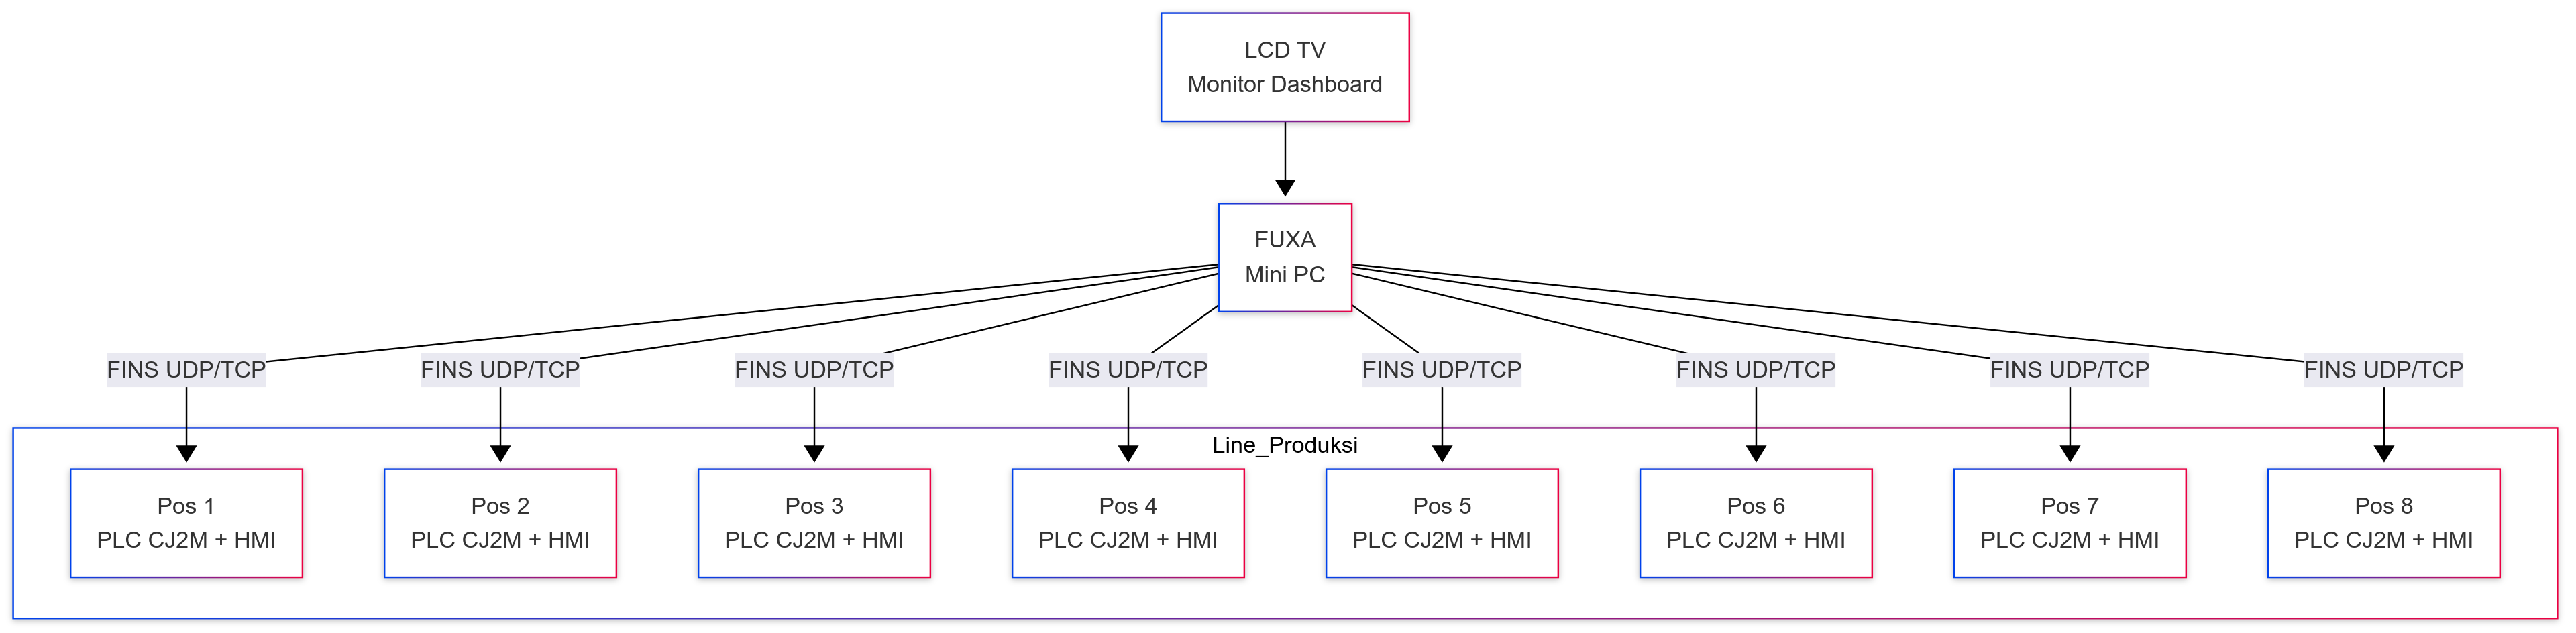
\includegraphics[width=\textwidth]{images/topologi_fuxa_fins.png} % Ganti dengan nama file SVG/PNG diagram hasil ekspor dari Mermaid
    \caption{Topologi Sistem SCADA FUXA dengan Protokol FINS}
    \label{fig:topologi}
\end{figure}

Diagram ini juga menunjukkan bahwa Mini PC berperan sebagai pusat kendali yang mengatur komunikasi ke setiap titik kontrol (posisi 1 sampai 8) di jalur produksi. Setiap posisi memiliki kombinasi PLC CJ2M dan HMI yang menangani proses otomatisasi lokal. Informasi yang dikumpulkan dan dianalisis oleh FUXA dapat disajikan secara waktu nyata melalui tampilan TV dashboard untuk kebutuhan pemantauan operator.

\section{Metode Pengujian}

Pengujian dilakukan untuk memastikan bahwa integrasi protokol FINS pada sistem SCADA FUXA berjalan dengan benar dan andal. Metode pengujian dibagi menjadi dua pendekatan utama, yaitu \textit{black-box testing} dan \textit{white-box testing}, sebagaimana dijelaskan berikut ini:

\subsection{Black-Box Testing}

Pengujian \textit{black-box} berfokus pada aspek fungsional sistem dari sudut pandang pengguna tanpa melihat struktur internal kode. Tujuan utama pengujian ini adalah untuk memverifikasi apakah sistem bekerja sesuai dengan yang diharapkan.

\begin{itemize}
    \item \textbf{Pengujian Konfigurasi Perangkat:} Memastikan bahwa parameter seperti \texttt{DA1}, \texttt{SA1}, \texttt{Unit Address}, dan \texttt{protocol} dapat disimpan dan ditampilkan ulang dengan benar.
    \item \textbf{Pengujian Pembacaan Data:} Mengamati apakah nilai dari PLC dapat ditampilkan di UI (user interface) FUXA secara waktu nyata setelah polling.
    \item \textbf{Pengujian Penulisan Data:} Menguji kemampuan sistem dalam mengubah nilai tag pada PLC dari UI, dan memastikan nilai benar-benar tersimpan di memori PLC.
    \item \textbf{Pengujian Alarm:} Mengaktifkan kondisi pemicu alarm dan mengevaluasi apakah notifikasi muncul sesuai logika yang ditetapkan.
    \item \textbf{Pengujian DAQ:} Memverifikasi apakah data historis disimpan dengan benar dalam sistem logging dan dapat ditampilkan kembali.
    \item \textbf{Pengujian Antarmuka:} Memastikan setiap komponen UI dapat diakses dan tidak menimbulkan error saat digunakan.
\end{itemize}

\subsection{White-Box Testing}

Pengujian \textit{white-box} dilakukan dengan menganalisis struktur internal dari sistem, termasuk logika program, alur data, serta penggunaan sumber daya. Pengujian ini membantu dalam menemukan error tersembunyi dan masalah performa.

\begin{itemize}
    \item \textbf{Unit Testing Konektor FINS:} Menguji fungsi-fungsi internal pada modul \texttt{server/runtime/devices/fins} seperti \texttt{connect()}, \texttt{read()}, \texttt{write()}, dan \texttt{poll()}.
    \item \textbf{Pengujian Event Emitter:} Mengevaluasi apakah listener pada konektor dibersihkan dengan benar untuk menghindari \textit{memory leak} akibat listener ganda.
    \item \textbf{Pengujian Error Handling:} Mengaktifkan simulasi gangguan komunikasi dan melihat apakah mekanisme retry atau error recovery berjalan dengan baik.
    \item \textbf{Logging dan Debug Output:} Memastikan bahwa log debug dapat memberikan informasi cukup untuk pelacakan kesalahan (tracing).
    \item \textbf{Pengamatan Trafik Jaringan:} Menggunakan Wireshark untuk memverifikasi bahwa paket FINS dikirim dan diterima sesuai dengan struktur protokol, termasuk header, command code, dan respons yang sesuai.
    \item \textbf{Integrasi Client-Server:} Menyusuri alur data dari UI (Angular) ke Node.js backend untuk menjamin komunikasi antar komponen berlangsung tanpa error.
\end{itemize}